\documentclass[a0paper,portrait]{baposter}



\usepackage{wrapfig}
\usepackage{lmodern}

\usepackage[utf8]{inputenc} %unicode support
\usepackage[T1]{fontenc}
\usepackage{hyperref}
\usepackage{xcolor}


\selectcolormodel{RGB}

\graphicspath{{figures/}} % Directory in which figures are stored


\newcommand{\compresslist}{%
\setlength{\itemsep}{0pt}%
\setlength{\parskip}{1pt}%
\setlength{\parsep}{0pt}%
}

\newenvironment{boenumerate}
  {\begin{enumerate}\renewcommand\labelenumi{\textbf\theenumi.}}
  {\end{enumerate}}



\begin{document}

\definecolor{loriapink}{RGB}{203,93,155}
\definecolor{loriablue}{RGB}{61,173,226}
\definecolor{loriadark}{RGB}{88,138,181}

\begin{poster}
{
grid=false,
headerborder=open, % Adds a border around the header of content boxes
colspacing=1em, % Column spacing
bgColorOne=white, % Background color for the gradient on the left side of the poster
bgColorTwo=white, % Background color for the gradient on the right side of the poster
borderColor=loriablue, % Border color
headerColorOne=loriadark, % Background color for the header in the content boxes (left side)
headerColorTwo=loriadark, % Background color for the header in the content boxes (right side)
headerFontColor=white, % Text color for the header text in the content boxes
boxColorOne=white, % Background color of the content boxes
textborder=rounded, %rectangle, % Format of the border around content boxes, can be: none, bars, coils, triangles, rectangle, rounded, roundedsmall, roundedright or faded
eyecatcher=false, % Set to false for ignoring the left logo in the title and move the title left
headerheight=0.11\textheight, % Height of the header
headershape=rounded, % Specify the rounded corner in the content box headers, can be: rectangle, small-rounded, roundedright, roundedleft or rounded
headershade=plain,
headerfont=\Large\textsf, % Large, bold and sans serif font in the headers of content boxes
%textfont={\setlength{\parindent}{1.5em}}, % Uncomment for paragraph indentation
linewidth=2pt % Width of the border lines around content boxes
}
{}
%
%----------------------------------------------------------------------------------------
%	TITLE AND AUTHOR NAME
%----------------------------------------------------------------------------------------
%
{\textsf{Controlled Conversational Models through \\ Conversation-Dedicated Ontology}}
{\sf\vspace{0.3em}\\
Barbara Gendron, under the supervision of Mathieu d'Aquin and Gaël Guibon
\vspace{0.1em}\\
\small{Laboratoire Lorrain de Recherche en Informatique et ses Applications (LORIA), Université de Lorraine
\vspace{0.2em}\\
barbara.gendron@loria.fr
}}
{
    \makebox[110pt][l]{
\includegraphics[width=0.15\textwidth]{all-logos.pdf}} 
}%

\headerbox{1. Context}{name=introduction,column=0,row=0, span=3}{

Recent advances in large language models (LLMs) have improved conversational agents' realism and acceptance. However, \textbf{controlling conversation flow towards positive outcomes remains crucial}. This Ph.D. aims to \textcolor{loriapink}{\bf represent conversational knowledge using an ontology to enable language model control}. Ontologies allow to model the knowledge in a domain, defining concepts and characterizing relations between them. While often used for domain-specific knowledge, few have explored using ontologies to guide conversation flow. Convology~\cite{convology} is a recent example focusing on managing health conversations. We plan to extend Convology's conceptualization capacities to a more general setup, therefore adaptable to general-purpose user/agent conversations.

}

\headerbox{Want to know more?}{name=resources,column=0,below=introduction,span=1}{

\begin{center}
    
\includegraphics[width=0.5\textwidth]{qrcode.jpg}\\
    My website, gh repo or whatever
\end{center}
}

\headerbox{2. Methodology}{name=method,column=0,below=resources,span=1}{

\paragraph*{PhD approach.} Iterative process by progressive enrichment of the ontology to conceptualize more and more notions related to conversations.\\
\paragraph*{Tools.} Protégé, HermiT and Pellet reasoners, owlready2, rdflib, PyTorch, huggingface transformers and parameter-efficient fine-tuning libraries, LoRA adapters.\\
\paragraph*{Conceptualization.} Explain our ontology engineering process and how we select and create toy examples.\\
\paragraph*{Control.} Explain how we plan to control the conversational dynamic inthe context of a dialogue user-agent.\\
\paragraph*{Challenges.} It is not straightforward that what the ontology brings can be fully understood and learnt by an LLM (in our case, we consider for now only decoder-based language models). 

\begin{center}
    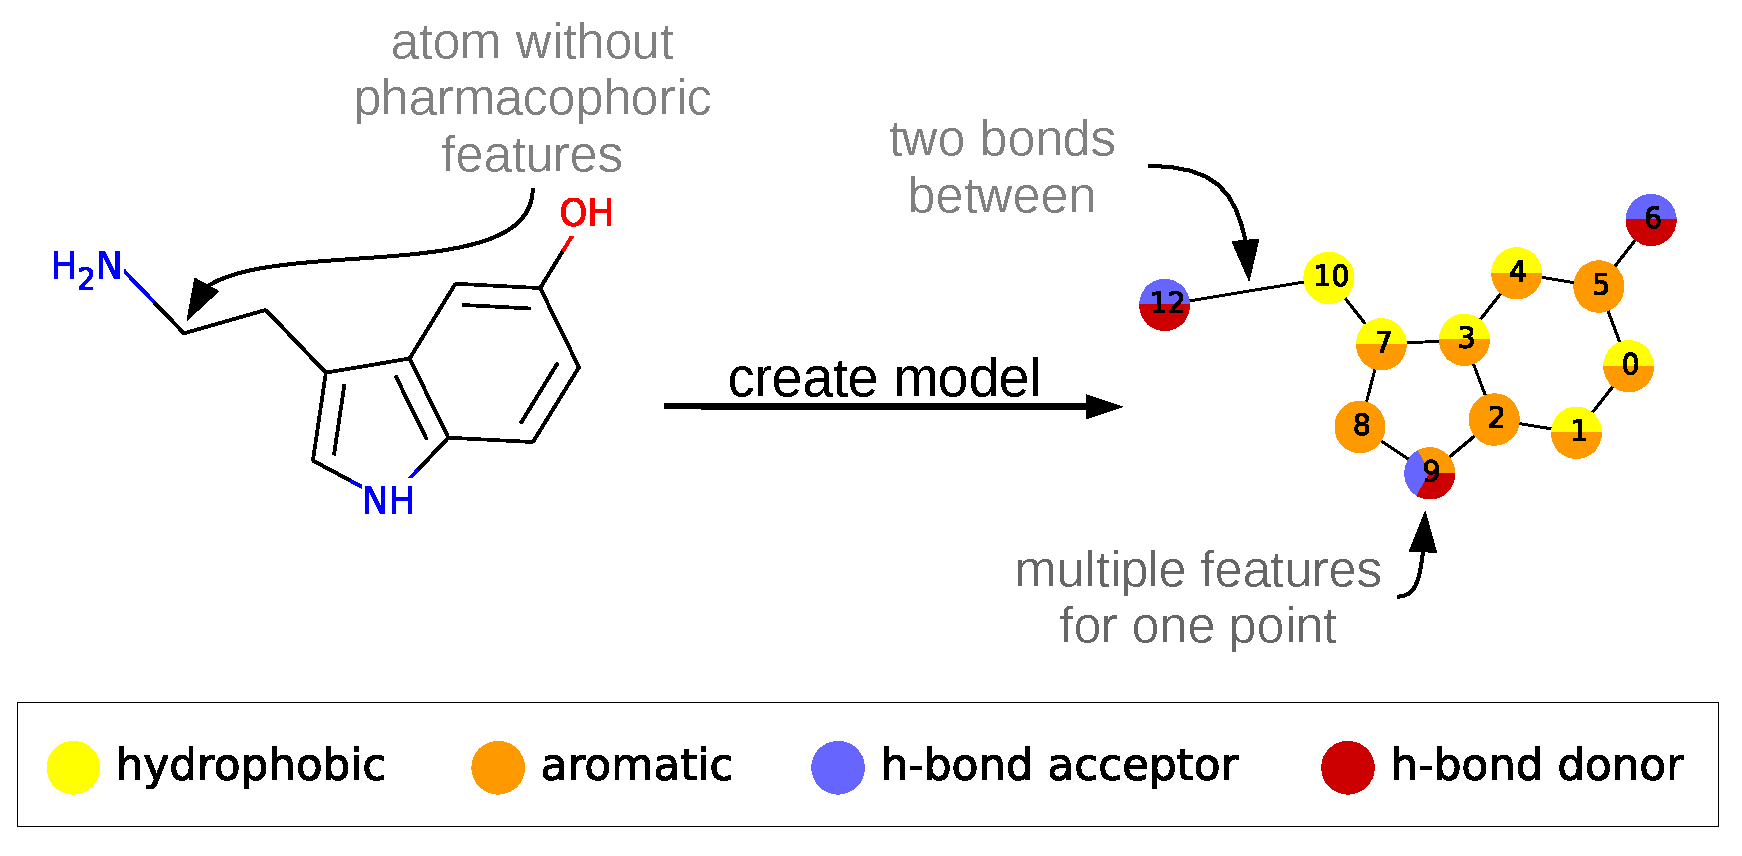
\includegraphics[width=\linewidth]{phar}
\end{center}
%\vspace{-2pt}
}

\headerbox{3. Objectives}{name=objectives,span=2,column=1,below=introduction}{ % To reduce this block to 1 column width, remove 'span=2'

\begin{wrapfigure}{l}{0.25\textwidth}
    \vspace{-15pt}
    \begin{center}
        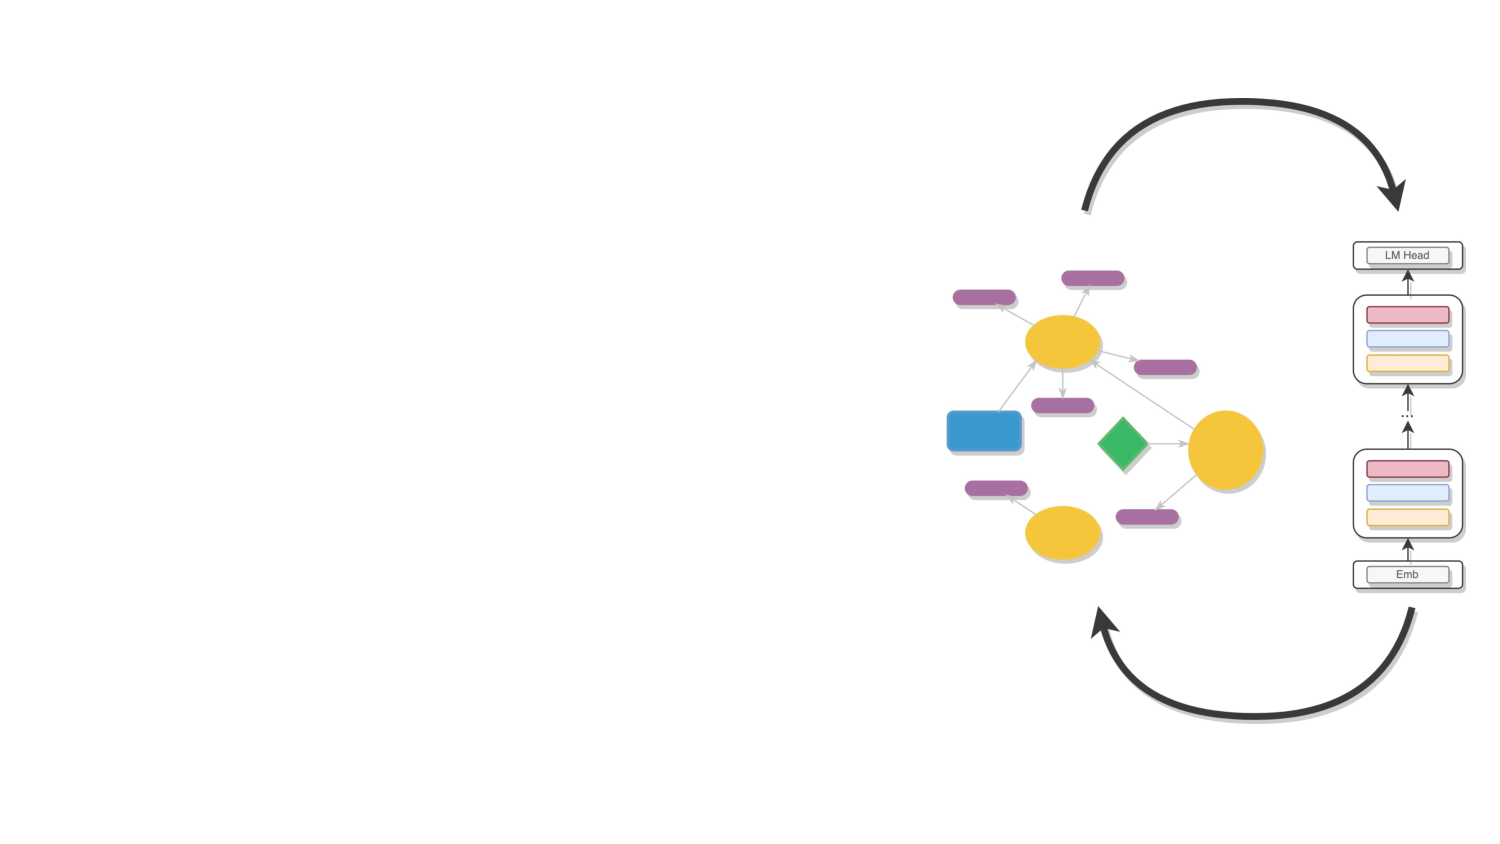
\includegraphics[width=\linewidth]{general-idea.pdf}
    \end{center}
\end{wrapfigure}
\vspace*{0.1em}
Develop \textbf{knowledge-enhanced conversational models} that exploit Large Language Models (LLMs) and Ontologies. The aim is to provide \textbf{structured knowledge} to open-domain conversational agents~\cite{varshney-first:2023}.

\begin{itemize}
    \item Build a conversation ontology that accounts for interpersonal relationships concepts and their evolution.
    \item Integrate and assess ontology understanding during fine-tuning.
    \item Bring control on conversational LLM outputs through encapsulated conversation knowledge.
\end{itemize}
\vspace*{0.3em}
}


\headerbox{4. OntoGPT: LLM Fine-Tuning Based on Ontology Validation}{name=ontogpt,span=2,column=1,below=objectives}{ % To reduce this block to 1 column width, remove 'span=2'
We work on a LLM/Ontology hybridation setup where the ontology is supposed to help the LLM produce more accurate utterances in dialogue (being as compliant as possible towards the user requirements). For this, we provide a an end-to-end integration pipeline where the ontology information is assimilated at fine-tuning time.

\begin{center}
    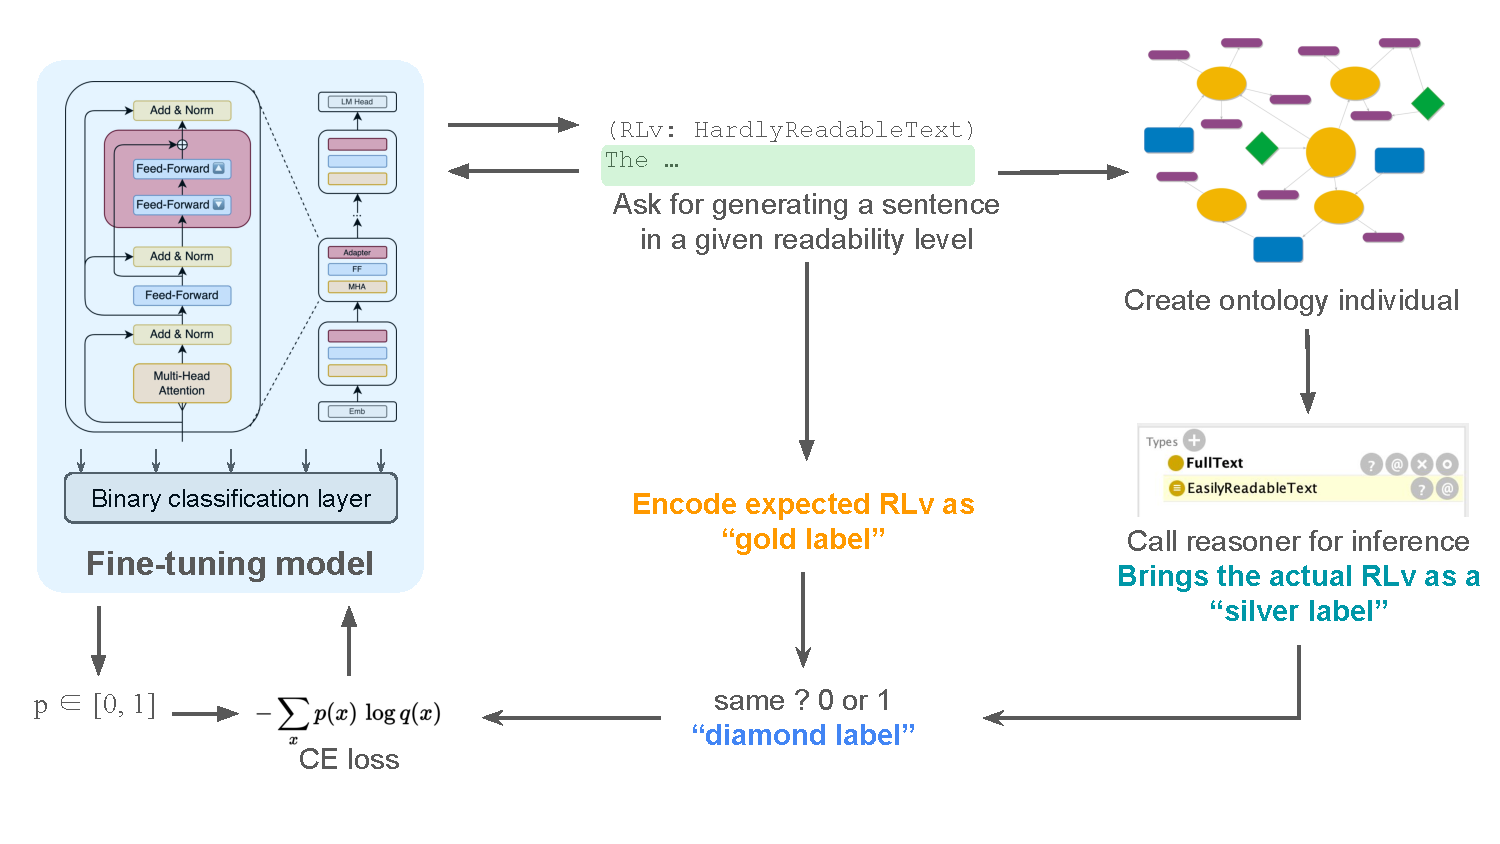
\includegraphics[width=0.95\linewidth]{ft-pipeline.pdf}
\end{center}
}


\headerbox{5. Related Work}{name=rwork,column=1,below=ontogpt,span=2}{
\begin{itemize}
    \item Many approaches use LLMs to improve KGs [Mateiu et al., 2023, He et al., 2023, Giglou et al., 2023] 
    \item “KGs to improve LLMs” approaches are less common but gain interest
    \begin{itemize}
        \item KG embeddings fed to BERT-like model [Gong et al., 2020]
        \item Integration of knowledge information using GANs [Varshney et al., 2023b]
        \item KLLM @ ACL 2024 (1st workshop on Knowledge Graphs and Large Language Models)
    \end{itemize}
\vspace*{2em}
\end{itemize} 
}


\headerbox{6. Selected references}{name=references,column=0,span=1,below=method,above=bottom}{

%\small % Reduce the font size in this block
\renewcommand{\section}[2]{\vskip 0.05em} % Get rid of the default "References" section title
%\nocite{*} % Insert publications even if they are not cited in the poster

\bibliographystyle{unsrt}
\bibliography{poster} % Use sample.bib as the bibliography file
}

\headerbox{7. Perpectives}{name=perspectives, column=1, span=2, below=rwork, above=bottom}{
We expect that the use of the ontology will also increase the interpretability of conversational agents, as decisions to use certain outputs over others will be associated with the ontological dimensions of the current conversation that have driven those choices, thus, moving from common fully black-box NLP models. This could also help these models be less harmful to both users and providers, along with controllable ethics in the way the conversation is analyzed.
}

\end{poster}

\end{document}
